\chapter{Implementacija i korisničko sučelje}
		
		
		\section{Korištene tehnologije i alati}
			
			\indent Pri izradi dokumentacije korišten je \textbf{LaTeX}\footnote{https://www.latex-project.org} - označni jezik korišten za uređivanje tekstualnih dokumenata najčešće znanstvene publikacije. Dokument je sastavljen u programu \textbf{TeXstudio}\footnote{https://www.texstudio.org} - uređivaču teksta prilagođen LaTeX-u. UML dijagrami nacrtani su uz pomoć alata \textbf{Astah UML}\footnote{https://astah.net/products/astah-uml}. Dijagrami koji nisu UML tipa nacrtani su u uređivaču \textbf{MS Word}\footnote{https://www.microsoft.com/en/microsoft-365/word}
			
			Udaljeni repozitorij projekta dostupan je na platformi \textbf{GitHub}\footnote{https://github.com}, korištenoj za pohranu svih datoteka potrebnih za rad na projektu.
			
			Za izradu pozadinskog dijela aplikacije korišten je objektno orijentirani programski jezik \textbf{Java}\footnote{https://www.java.com/en} i radni okvir \textbf{Spring Boot}\footnote{https://spring.io/projects/spring-boot} - specijalizacija radnog okvira Spring, s ciljem jednostavnijeg i bržeg oblikovanja web aplikacije. Kao razvojno okruženje korišten je \textbf{IntelliJ IDEA}\footnote{https://www.jetbrains.com/idea}. Tijekom izrade, pozadinski dio aplikacije testiran je pomoću platforme za testiranje API-ja \textbf{Postman}\footnote{https://www.postman.com}.
			
			Za izradu prednjeg dijela aplikacije korišten je \textbf{React}\footnote{https://react.dev} i JavaScript ekstenzija \textbf{JavaScript XML}\footnote{https://legacy.reactjs.org/docs/introducing-jsx.html}. React, također poznat kao React.js ili ReactJS, je biblioteka u JavaScriptu za izgradnju korisničkih sučelja koju održava \textit{Facebook}. \textit{React} se najčešće koristi kao osnova u razvoju mrežnih ili mobilnih aplikacija. Složene aplikacije u \textit{React}-u obično zahtijevaju korištenje dodatnih biblioteka za interakciju s API-jem.
			
			Baza podataka izrađena je u sustavu za upravljanje bazama podataka \textbf{PostgreSQL}\footnote{https://www.postgresql.org}. Za pristup PostgreSQL sustavu baze podataka korišten je \textbf{pgAdmin 4}\footnote{https://www.pgadmin.org} program. Za izradu ER dijagrama baze podataka korišten je \textbf{ERDPlus}\footnote{https://erdplus.com} alat.
			
			Aplikacija i baza podataka su postavljene na udaljene poslužitelje kao usluga aplikacije \textbf{Render}\footnote{https://render.com}, koja nudi besplatnu opciju pri iznajmljivanju sklopovlja, s ograničenim mogućnostima.
			
			Komunikacija između članova tima ostvarena je putem aplikacija s tom svrhom: \textbf{WhatsApp}\footnote{https://www.whatsapp.com} i \textbf{Discord}\footnote{https://discord.com}.
			
			\eject 
		
	
		\section{Ispitivanje programskog rješenja}	 
			
			\subsection{Ispitivanje komponenti}
			\textit{Potrebno je provesti ispitivanje jedinica (engl. unit testing) nad razredima koji implementiraju temeljne funkcionalnosti. Razraditi \textbf{minimalno 6 ispitnih slučajeva} u kojima će se ispitati redovni slučajevi, rubni uvjeti te izazivanje pogreške (engl. exception throwing). Poželjno je stvoriti i ispitni slučaj koji koristi funkcionalnosti koje nisu implementirane. Potrebno je priložiti izvorni kôd svih ispitnih slučajeva te prikaz rezultata izvođenja ispita u razvojnom okruženju (prolaz/pad ispita). }
			
			Ispitivanje komponenti provedeno je pomoću Selenium WebDrivera\footnote{https://www.selenium.dev/documentation/webdriver/} unutar JUnit 4 testova kao podršku za pisanje ispita unutar programskog jezika Java. Ispitivanje je provedeno nad konferencijom naziva "TestKonferencija". U vrijeme izrade dokumentacije, konferencija se nalazila na drugom mjestu na listi dostupnih konferencija. 
			Izrađeno je 7 ispitnih slučajeva. Uspješnost 6 slučajeve te izazivanje pogreške u jednom prikazani su slikom 5.1.
			
			\begin{figure} [hbt!]
				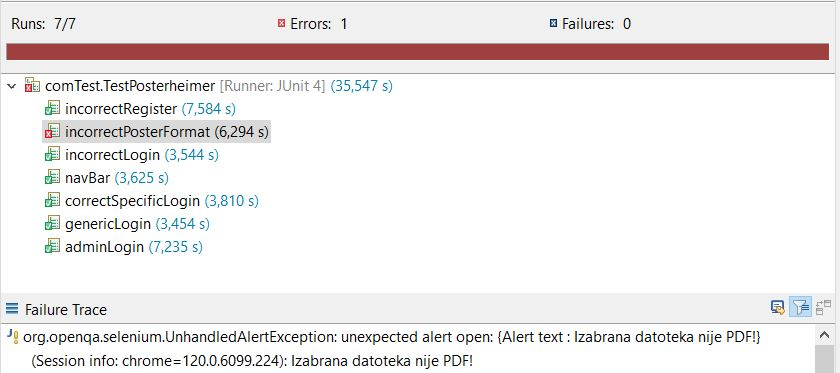
\includegraphics[width=\linewidth]{Slike/testResults}
				\caption{Prikaz uspješnosti ispitnih slučajeva}
			\end{figure}
			
			\newpage
			
			U \textbf{prvom ispitnom slučaju} provjerena je funkcionalnost gumba za pristup konferenciji pri inicijalnom pristupu pomoću točnog generičkog korisničkog imena (adrese e-pošte predviđenu za generički račun) i odgovarajuće lozinke. Predviđen rezultat je dozvoljen pristup stranici konferencije. Ispitni slučaj je uspješan.
			
			
			\begin{lstlisting}
@Test
public void genericLogin() {
	
	System.setProperty("webdriver.chrome.driver", "src\\test\\java\\chromedriver\\chromedriver.exe");
	WebDriver driver = new ChromeDriver();
	driver.manage().timeouts().implicitlyWait(10, TimeUnit.SECONDS);
	
	driver.get("https://posterheimer.onrender.com/");
	org.openqa.selenium.Dimension target = new  org.openqa.selenium.Dimension(1552, 840);
	driver.manage().window().setSize(target);
	
	driver.findElement(By.xpath("(//button[contains(text(),'Pristupi')])[2]")).click();
	// broj postaviti na mjesto konferencije u listi
	
	driver.findElement(By.id("username")).click();
	driver.findElement(By.id("username")).sendKeys("visitor.test@mail.hr");
	driver.findElement(By.id("password")).click();
	driver.findElement(By.id("password")).sendKeys("Lozinka1");
	driver.findElement(By.cssSelector(".btn-primary")).click();
	
	driver.findElement(By.linkText("Konferencija")).click();
	
	String redirURL = driver.getCurrentUrl();
	boolean comperRes = redirURL.contains("/conference");
	if(comperRes == true) {
		System.out.println("Pristupljeno konferenciji");
	} else {
		System.out.println("Error");
	}
	assertEquals(comperRes, true);
	driver.quit();
}
			\end{lstlisting}
			
			U \textbf{drugom ispitnom slučaju} provjerena je funkcionalnost gumba za pristup konferenciji pomoću jedinstvenog korisničkog računa, te odjava. Potrebno je upisati točnu adresu e-pošte i odgovarajuću lozinku već stvorenog korisničkog računa. Nakon upisa podataka, korisnik dobiva pristup stranici konferencije. Nakon prijave, korisnik se odjavljuje. Predviđen rezultat je povratak na početnu stranicu aplikacije. Ispitni slučaj je uspješan.  

			
			\begin{lstlisting}
@Test
public void correctSpecificLogin() {
	System.setProperty("webdriver.chrome.driver", "src\\test\\java\\chromedriver\\chromedriver.exe");
	WebDriver driver = new ChromeDriver();
	driver.manage().timeouts().implicitlyWait(10, TimeUnit.SECONDS);
	
	driver.get("https://posterheimer.onrender.com/");
	driver.manage().window().setSize(new Dimension(1552, 840));
	driver.findElement(By.cssSelector(".list-group-item:nth-child(4) > .float-end")).click();
	driver.findElement(By.id("username")).click();
	driver.findElement(By.id("username")).sendKeys("register.email@mail.hr");
	driver.findElement(By.id("password")).click();
	driver.findElement(By.id("password")).sendKeys("Lozinka1");
	driver.findElement(By.cssSelector(".btn-primary")).click();
	
	driver.findElement(By.linkText("Konferencija")).click();
	
	String redirURL = driver.getCurrentUrl();
	boolean comperRes = redirURL.contains("/conference");
	if(comperRes == true) {
		System.out.println("Pristupljeno konferenciji");
	} else {
		System.out.println("Error: prijava");
	}
	
	driver.findElement(By.id("user-dropdown")).click();
	driver.findElement(By.cssSelector(".fa-right-from-bracket")).click();
	
	redirURL = driver.getCurrentUrl();
	comperRes = redirURL.equals("https://posterheimer.onrender.com/");
	if(comperRes == true) {
		System.out.println("Ostvarena odjava");
	} else {
		System.out.println("Error: odjava");
	}
	driver.quit();
}	
			\end{lstlisting}
			
			
			U \textbf{trećem ispitnom slučaju} provjerena je funkcionalnost gumba za pristup konferenciji pri neispravnoj prijavi. Predviđen rezultat je prikaz obavijesti "Pogrešan email ili lozinka!" te ostajanje na sučelju za prijavu unutar početne stranice. Ispitni slučaj je uspješan.
			
			\begin{lstlisting}
@Test
public void incorrectLogin() {
	System.setProperty("webdriver.chrome.driver", "src\\test\\java\\chromedriver\\chromedriver.exe");
	WebDriver driver = new ChromeDriver();
	driver.manage().timeouts().implicitlyWait(10, TimeUnit.SECONDS);
	
	driver.get("https://posterheimer.onrender.com/");
	driver.manage().window().setSize(new Dimension(1552, 840));
	driver.findElement(By.xpath("(//button[@type=\'button\'])[2]")).click(); // vrijednost koju mijenjamo

	driver.findElement(By.cssSelector(".mb-3:nth-child(1)")).click();
	driver.findElement(By.id("username")).click();
	driver.findElement(By.id("username")).sendKeys("test");
	driver.findElement(By.id("password")).click();
	driver.findElement(By.id("password")).sendKeys("test");
	driver.findElement(By.cssSelector(".btn-primary")).click();
	
	driver.findElement(By.cssSelector(".alert")).click();

	WebElement alert = driver.findElement(By.cssSelector(".alert"));
	String errorMessage = alert.getText();
	if(errorMessage.contains("email ili lozinka!")) {
		System.out.println("Prikaz prikladne obavijesti");
	}
	
	driver.findElement(By.cssSelector(".btn-close")).click();
	
	String redirURL = driver.getCurrentUrl();
	boolean comperRes = redirURL.equals("https://posterheimer.onrender.com/");
	if(comperRes) {
		System.out.println("Ostvaren rezultat");
	}
	driver.quit();
}
			\end{lstlisting}
			
			Neispravnu prijavu ispitati ćemo i pomoću postojećeg korisničkog računa koji nije namijenjen odabranoj konferenciji. Upisat ćemo redni broj druge konferencije, kao \textit{username} poslati "visitor.test@mail.hr" te "Lozinka1" za \textit{password}. Predviđeni rezultat je ponovan prikaz obavijesti "Pogrešan email ili lozinka!". Ispitni slučaj nije uspješan - obavijest se ne prikazuje te je korisniku dozvoljen pristup konferenciji. Funkcionalnost bi u budućnosti trebalo implementirati.
			
			\begin{figure} [hbt!]
				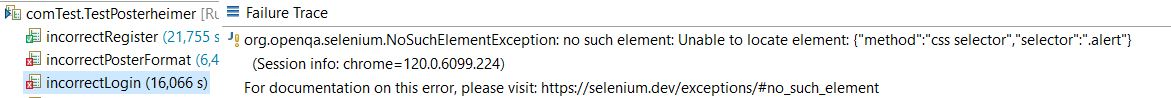
\includegraphics[width=\linewidth]{Slike/incorrectLoginFail}
				\caption{Prikaz pada ispitnog slučaja}
			\end{figure}
			
			
			
			U \textbf{četvrtom ispitnom slučaju} provjerena je funkcionalnost gumba za pristup konferenciji pri prijavi administratora. Predviđen rezultat je dozvoljen pristup konferenciji, te mogućnost dodavanja postera, fotografija i pokrovitelja. Ispitni slučaj je uspješan.
			
			\begin{lstlisting}
@Test
public void adminLogin() {
	System.setProperty("webdriver.chrome.driver", "src\\test\\java\\chromedriver\\chromedriver.exe");
	WebDriver driver = new ChromeDriver();
	driver.manage().timeouts().implicitlyWait(20, TimeUnit.SECONDS);
	// Vrijeme povecano zbog ucitavanja postera, koje je znatno sporije za administratora
	
	driver.get("https://posterheimer.onrender.com/");
	driver.manage().window().setSize(new Dimension(1552, 840));
	driver.findElement(By.cssSelector(".list-group-item:nth-child(2) > .float-end")).click();
	driver.findElement(By.id("username")).click();
	driver.findElement(By.id("username")).sendKeys("admin.test@mail.hr");
	driver.findElement(By.id("password")).click();
	driver.findElement(By.id("password")).sendKeys("Lozinka1");
	driver.findElement(By.cssSelector(".btn-primary")).click();
	driver.findElement(By.cssSelector(".conference-content")).click();
	driver.findElement(By.linkText("Posteri")).click();
	driver.findElement(By.cssSelector(".fa-solid")).click();
	driver.findElement(By.cssSelector(".btn-close")).click();
	driver.findElement(By.linkText("Fotografije")).click();
	driver.findElement(By.cssSelector(".image-container > img")).click();
	driver.findElement(By.cssSelector(".modal-title")).click();
	driver.findElement(By.cssSelector(".btn-close")).click();
	driver.findElement(By.linkText("Pokrovitelji")).click();
	driver.findElement(By.cssSelector(".fa-solid")).click();
	driver.findElement(By.cssSelector(".modal-title")).click();
	driver.findElement(By.cssSelector(".btn-close")).click();
	
	String redirURL = driver.getCurrentUrl();
	boolean comperRes = redirURL.contains("sponsors");
	if(comperRes) {
		System.out.println("Ostvaren rezultat");
	}
	driver.quit();
}
			\end{lstlisting}
			
	\newpage
			
	U \textbf{petom ispitnom slučaju} provjerena je funkcionalnost navigacijske trake. Predviđen rezultat je otvaranje stranice konferencije nakon klika na "Konferencija", stranice postera nakon klika na "Posteri", stranice za fotografije nakon klika na "Fotografije" i stranice pokrovitelja nakon klika na "Pokrovitelji". Ispitni slučaj je uspješan.
	
	\begin{lstlisting}
@Test
public void navBar() {
	System.setProperty("webdriver.chrome.driver", "src\\test\\java\\chromedriver\\chromedriver.exe");
	WebDriver driver = new ChromeDriver();
	driver.manage().timeouts().implicitlyWait(10, TimeUnit.SECONDS);	
	
	driver.get("https://posterheimer.onrender.com/");
	org.openqa.selenium.Dimension target = new  org.openqa.selenium.Dimension(1552, 840);
	driver.manage().window().setSize(target);
	
	driver.findElement(By.xpath("(//button[contains(text(),'Pristupi')])[2]")).click();
	// broj postaviti na mjesto konferencije u listi
	
	driver.findElement(By.id("username")).click();
	driver.findElement(By.id("username")).sendKeys("visitor.test@mail.hr");
	driver.findElement(By.id("password")).click();
	driver.findElement(By.id("password")).sendKeys("Lozinka1");
	driver.findElement(By.cssSelector(".btn-primary")).click();
	
	driver.findElement(By.linkText("Konferencija")).click();
	String redirURL = driver.getCurrentUrl();
	boolean comperRes = redirURL.contains("/conference");
	if(comperRes == true) {
		System.out.println("Pristupljeno konferenciji");
	} else {
		System.out.println("Error: konferencije");
	}
	
	driver.findElement(By.linkText("Posteri")).click();
	redirURL = driver.getCurrentUrl();
	comperRes = redirURL.contains("/posters");
	if(comperRes == true) {
		System.out.println("Pristupljeno posterima");
	} else {
		System.out.println("Error: posteri");
	}
	
	driver.findElement(By.linkText("Fotografije")).click();
	redirURL = driver.getCurrentUrl();
	comperRes = redirURL.contains("/photos");
	if(comperRes == true) {
		System.out.println("Pristupljeno fotografijama");
	} else {
		System.out.println("Error: fotografije");
	}
	driver.findElement(By.linkText("Pokrovitelji")).click();
	redirURL = driver.getCurrentUrl();
	comperRes = redirURL.contains("/sponsors");
	if(comperRes == true) {
		System.out.println("Pristupljeno pokroviteljima");
	} else {
		System.out.println("Error: pokrovitelji");
	}
	
	/* ukoliko je glasovanje gotovo
	driver.findElement(By.linkText("Rezultati")).click();
	redirURL = driver.getCurrentUrl();
	comperRes = redirURL.contains("/results");
	if(comperRes == true) {
		System.out.println("Pristupljeno rezultatima");
	} else {
		System.out.println("Error: rezultati");
	}
	*/
	driver.quit();
}
	\end{lstlisting}
	
	U \textbf{šestom ispitnom slučaju} provjerena je funkcionalnost gumba za registraciju pri unosu adrese e-pošte netočnog formata. Sva ostala polja su točno ispunjena, a reCAPTCHA test je prošao. Predviđen rezultat je neuspješna registracija te obavijest o netočnom unosu. Ispitni slučaj je uspješan.
	Ispitni slučaj je neuspješan u slučaju CAPTCHA Image testa 

			\begin{lstlisting}
@Test
public void incorrectRegister() {
	System.setProperty("webdriver.chrome.driver", "src\\test\\java\\chromedriver\\chromedriver.exe");
	WebDriver driver = new ChromeDriver();
	JavascriptExecutor js = (JavascriptExecutor) driver;
	driver.manage().timeouts().implicitlyWait(10, TimeUnit.SECONDS);
	
	driver.get("https://posterheimer.onrender.com/");
	driver.manage().window().setSize(new Dimension(1552, 840));
	driver.findElement(By.cssSelector(".list-group-item:nth-child(2) > .float-end")).click();
	driver.findElement(By.cssSelector("form")).click();
	driver.findElement(By.id("username")).click();
	driver.findElement(By.id("username")).sendKeys("visitor.test@mail.hr");
	driver.findElement(By.id("password")).click();
	driver.findElement(By.id("password")).sendKeys("Lozinka1");
	driver.findElement(By.cssSelector(".btn-primary")).click();
	driver.findElement(By.linkText("Registracija")).click();
	js.executeScript("window.scrollTo(0,0)");
	driver.findElement(By.id("formIme")).click();
	driver.findElement(By.id("formIme")).sendKeys("TestIme");
	driver.findElement(By.id("formPrezime")).click();
	driver.findElement(By.id("formPrezime")).sendKeys("TestPrezime");
	driver.findElement(By.id("formBasicEmail")).click();
	driver.findElement(By.id("formBasicEmail")).sendKeys("email");
	driver.findElement(By.id("formBasicPassword")).click();
	driver.findElement(By.id("formBasicPassword")).sendKeys("lozinka");
	driver.findElement(By.cssSelector(".mb-3:nth-child(2) > #formBasicPassword")).click();
	driver.findElement(By.cssSelector(".mb-3:nth-child(2) > #formBasicPassword")).sendKeys("lozinka");
	driver.switchTo().frame(0);
	driver.findElement(By.cssSelector(".recaptcha-checkbox-border")).click();
	driver.switchTo().defaultContent();
	driver.findElement(By.cssSelector(".ml-2")).click();
	driver.findElement(By.cssSelector(".mx-2 > .mb-3:nth-child(1)")).click();
	driver.findElement(By.cssSelector(".mx-2 > .mb-3:nth-child(1)")).click();
	
	String redirURL = driver.getCurrentUrl();
	boolean comperRes = redirURL.contains("/register");
	if(comperRes == true) {
		System.out.println("Neuspjesna registracija");
	} else {
		System.out.println("Error");
	}
	
	driver.quit();
}	  
			\end{lstlisting}
			
		U \textbf{sedmom ispitnom slučaju} provjerena je funkcionalnost sučelja za dodavanje postera pri unosu datoteke netočnog formata. Prije dodavanja postera potrebna je prijava administratora. Predviđen rezultat je prikaz obavijesti "Izabrana datoteka nije PDF!". Rezultat je ostvaren.  
		
	\begin{lstlisting}
@Test
public void incorrectPosterFormat() {
	System.setProperty("webdriver.chrome.driver", "src\\test\\java\\chromedriver\\chromedriver.exe");
	WebDriver driver = new ChromeDriver();
	JavascriptExecutor js = (JavascriptExecutor) driver;
	File filepath = new File("src\\test\\java\\files\\example.pptx");
	
	
	driver.manage().timeouts().implicitlyWait(10, TimeUnit.SECONDS);
	
	
	driver.get("https://posterheimer.onrender.com/");
	driver.manage().window().setSize(new Dimension(1552, 840));
	driver.findElement(By.cssSelector(".list-group-item:nth-child(2) > .float-end")).click();	  
	
	driver.findElement(By.id("username")).click();
	driver.findElement(By.id("username")).sendKeys("admin.test@mail.hr");
	driver.findElement(By.id("password")).click();
	driver.findElement(By.id("password")).sendKeys("Lozinka1");
	driver.findElement(By.cssSelector(".btn-primary")).click();
	driver.findElement(By.linkText("Posteri")).click();
	driver.findElement(By.cssSelector(".fa-solid")).click();
	
	WebElement fileInput = driver.findElement(By.cssSelector("input[type=file]"));
	fileInput.sendKeys(filepath.getAbsolutePath());
	
	driver.findElement(By.name("imePoster")).click();
	driver.findElement(By.name("imePoster")).sendKeys("Krivi format");
	driver.findElement(By.name("imeAutor")).click();
	driver.findElement(By.name("imeAutor")).sendKeys("Ime");
	driver.findElement(By.name("prezimeAutor")).click();
	driver.findElement(By.name("prezimeAutor")).sendKeys("Prezime");
	driver.findElement(By.cssSelector("form")).click();
	driver.findElement(By.name("posterEmail")).click();
	driver.findElement(By.name("posterEmail")).sendKeys("test.poster@posterheimer.hr");
	driver.findElement(By.cssSelector(".btn")).click();
	
	WebElement alert = driver.findElement(By.cssSelector(".alert"));
	String errorMessage = alert.getText();
	if(errorMessage.contains("Izabrana datoteka nije PDF!")) {
		System.out.println("Prikaz prikladne obavijesti");
	} else {
		System.out.println("Error");
	}		
	
	driver.findElement(By.cssSelector(".alert")).click();
	driver.findElement(By.cssSelector(".btn-close")).click();
	
	
	driver.quit();
}
	\end{lstlisting}
	
			\newpage
			
			\subsection{Ispitivanje sustava}
		 	
		 	Ispitivanje sustava provedeno je pomoću dodatka za preglednik Selenium IDE\footnote{https://www.selenium.dev/selenium-ide/}. JUnit ispitni slučajevi generirani su pomoću Selenium IDE ispitnih slučajeva.
		 	
		 	\textbf{Prvi ispitni slučaj} provjerava funkcionalnost brisanja korisnika. Prije brisanja korisnika potrebna je prijava registratora. Administrator briše određenog korisnika te se odjavljuje. Uspješnost brisanja korisnika provjeravamo pokušajem prijave izbrisanog korisnika. Očekivani rezultat je neuspješna prijava. Ispitni slučaj je uspješan.
		 	
		 	\begin{figure} [hbt!]
		 		\includegraphics[width=\linewidth]{Slike/deleteUser}
		 		\caption{Prikaz uspješnosti ispitnog slučaja}
		 	\end{figure}
		 	
		\begin{lstlisting}
  @Test
public void deleteUser() {
	driver.get("https://posterheimer.onrender.com/");
	driver.manage().window().setSize(new Dimension(1552, 840));
	driver.findElement(By.cssSelector(".list-group-item:nth-child(5) > .float-end")).click();
	{
		WebElement element = driver.findElement(By.cssSelector(".list-group-item:nth-child(5) > .float-end"));
		Actions builder = new Actions(driver);
		builder.moveToElement(element).perform();
	}
	{
		WebElement element = driver.findElement(By.tagName("body"));
		Actions builder = new Actions(driver);
		builder.moveToElement(element, 0, 0).perform();
	}
	driver.findElement(By.cssSelector(".mb-3:nth-child(1)")).click();
	driver.findElement(By.id("username")).click();
	driver.findElement(By.id("username")).sendKeys("admin.test@mail.hr");
	driver.findElement(By.cssSelector("form")).click();
	driver.findElement(By.id("password")).click();
	driver.findElement(By.id("password")).sendKeys("pass");
	driver.findElement(By.cssSelector(".btn-primary")).click();
	driver.findElement(By.id("user-dropdown")).click();
	driver.findElement(By.linkText("Korisnici")).click();
	driver.findElement(By.cssSelector(".list-group-item:nth-child(16) > .float-start")).click();
	driver.findElement(By.id("root")).click();
	driver.findElement(By.cssSelector(".list-group-item:nth-child(18) > .btn")).click();
	driver.findElement(By.id("user-dropdown")).click();
	driver.findElement(By.linkText("Odjava")).click();
	driver.findElement(By.cssSelector(".list-group-item:nth-child(5) > .float-end")).click();
	{
		WebElement element = driver.findElement(By.cssSelector(".list-group-item:nth-child(5) > .float-end"));
		Actions builder = new Actions(driver);
		builder.moveToElement(element).perform();
	}
	{
		WebElement element = driver.findElement(By.tagName("body"));
		Actions builder = new Actions(driver);
		builder.moveToElement(element, 0, 0).perform();
	}
	driver.findElement(By.id("username")).click();
	driver.findElement(By.id("username")).sendKeys("register2.");
	driver.findElement(By.id("username")).sendKeys("register2.email@mail.hr");
	driver.findElement(By.id("password")).click();
	driver.findElement(By.id("password")).sendKeys("pass");
	driver.findElement(By.cssSelector(".btn-primary")).click();
}
		\end{lstlisting}
		
\newpage
		
\textbf{Drugi ispitni slučaj} provjerava funkcionalnost gumba za registraciju pri unosu podataka ispravnog formata. Tijekom registracije odabrana je opcija "Prikaz lozinke" te prođen CAPTCHA test. Rezultat ispitnog slučaja je uspješan.

\begin{figure} [hbt!]
	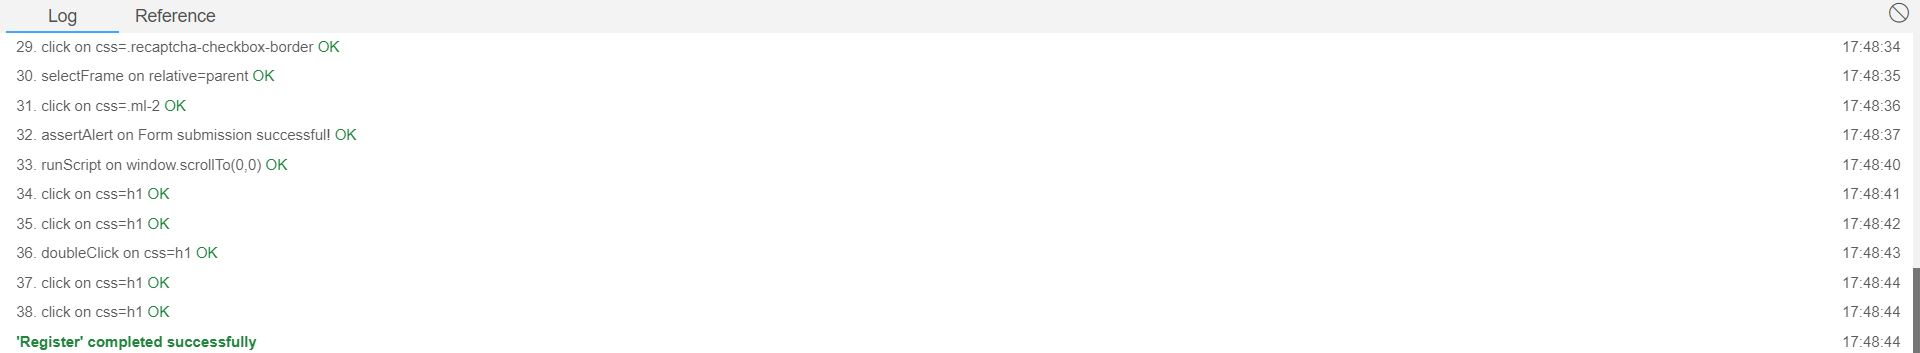
\includegraphics[width=\linewidth]{Slike/Register}
	\caption{Prikaz uspješnosti ispitnog slučaja}
\end{figure}

\begin{lstlisting}
	@Test
	public void register() {
		driver.get("https://posterheimer.onrender.com/");
		driver.manage().window().setSize(new Dimension(1552, 840));
		driver.findElement(By.cssSelector(".list-group-item:nth-child(5) > .float-end")).click();
		driver.findElement(By.id("username")).click();
		driver.findElement(By.id("username")).sendKeys("visitor.test@mail.hr");
		driver.findElement(By.id("password")).click();
		driver.findElement(By.id("password")).sendKeys("pass");
		driver.findElement(By.cssSelector(".btn-primary")).click();
		driver.findElement(By.cssSelector(".conference-content")).click();
		driver.findElement(By.cssSelector(".mx-auto:nth-child(1)")).click();
		driver.findElement(By.cssSelector(".card-text")).click();
		driver.findElement(By.linkText("Registracija")).click();
		js.executeScript("window.scrollTo(0,0)");
		driver.findElement(By.id("formIme")).click();
		driver.findElement(By.id("formIme")).sendKeys("TestIme");
		driver.findElement(By.id("formPrezime")).click();
		driver.findElement(By.id("formPrezime")).sendKeys("TestPrezime");
		driver.findElement(By.id("formBasicEmail")).click();
		driver.findElement(By.id("formBasicEmail")).click();
		driver.findElement(By.id("formBasicEmail")).sendKeys("register.email@mail.hr"); // promijeniti email za svaki test
		driver.findElement(By.id("formBasicPassword")).click();
		driver.findElement(By.id("formBasicPassword")).sendKeys("pass");
		driver.findElement(By.cssSelector(".mb-3:nth-child(2) > #formBasicPassword")).click();
		driver.findElement(By.cssSelector(".mb-3:nth-child(2) > #formBasicPassword")).sendKeys("pass");
		driver.findElement(By.cssSelector(".form-check")).click();
		driver.findElement(By.id("formShowPassword")).click();
		driver.findElement(By.id("formShowPassword")).click();
		driver.switchTo().frame(0);
		driver.findElement(By.cssSelector(".recaptcha-checkbox-border")).click();
		driver.switchTo().defaultContent();
		driver.findElement(By.cssSelector(".ml-2")).click();
		assertThat(driver.switchTo().alert().getText(), is("Form submission successful!"));
		js.executeScript("window.scrollTo(0,0)");
		driver.findElement(By.cssSelector("h1")).click();
		driver.findElement(By.cssSelector("h1")).click();
		{
			WebElement element = driver.findElement(By.cssSelector("h1"));
			Actions builder = new Actions(driver);
			builder.doubleClick(element).perform();
		}
		driver.findElement(By.cssSelector("h1")).click();
		driver.findElement(By.cssSelector("h1")).click();
	}
\end{lstlisting}

\textbf{Treći ispitni slučaj} provjerava funkcionalnost gumba za dodavanje konferencije. Prije dodavanja konferencije potrebna je prijava natkorisnika. Podaci vezani za korisnički račun natkorisnika uklonjeni su iz izvornog koda. Predviđen rezultat  je stvaranje nove konferencije. Ispitni slučaj je uspješan.

\begin{figure} [hbt!]
	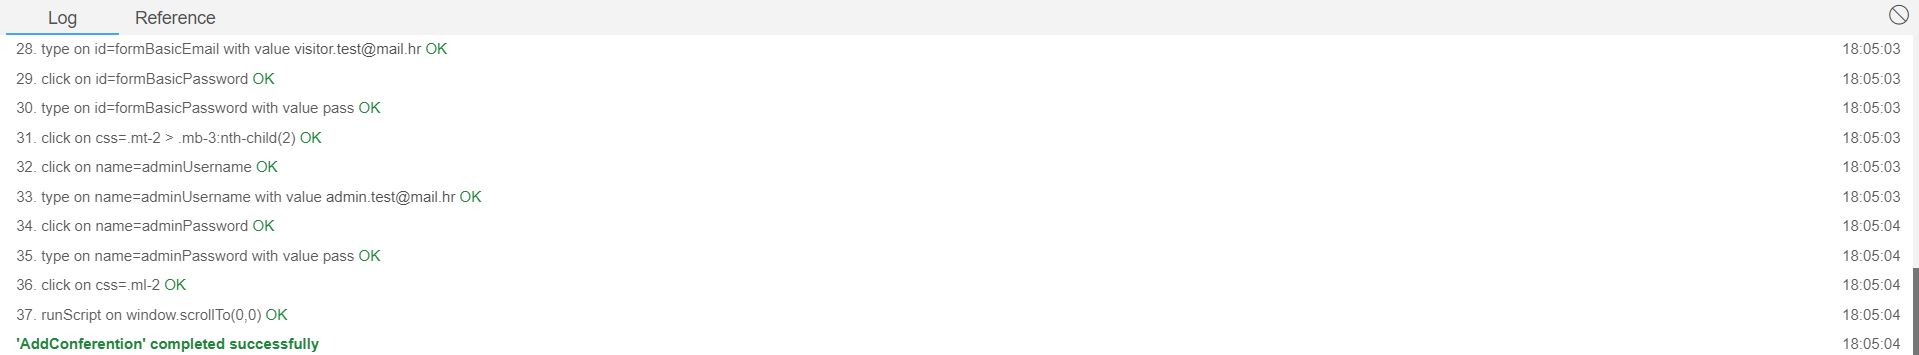
\includegraphics[width=\linewidth]{Slike/addConferention}
	\caption{Prikaz uspješnosti ispitnog slučaja}
\end{figure}

\begin{lstlisting}
	@Test
	public void addConferention() {
		driver.get("https://posterheimer.onrender.com/");
		driver.manage().window().setSize(new Dimension(1552, 840));
		driver.findElement(By.cssSelector(".fa-solid")).click();
		driver.findElement(By.id("username")).click();
		driver.findElement(By.id("username")).sendKeys("ime natkorisnika");
		driver.findElement(By.id("password")).click();
		driver.findElement(By.id("password")).sendKeys("lozinka natkorisnika");
		driver.findElement(By.cssSelector(".btn-primary")).click();
		driver.findElement(By.cssSelector(".fa-square-plus")).click();
		driver.findElement(By.id("formConferenceName")).click();
		driver.findElement(By.id("formConferenceName")).sendKeys("AutomaticTestKonferencija");
		driver.findElement(By.name("videoUrl")).click();
		driver.findElement(By.name("videoUrl")).sendKeys("https://www.youtube.com/watch?v=ScMzIvxBSi4&ab_channel=BenMarquezTX");
		driver.findElement(By.id("formConferenceCity")).click();
		driver.findElement(By.id("formConferenceCity")).sendKeys("Unska ");
		driver.findElement(By.id("formConferenceCity")).sendKeys("Unska 3");
		driver.findElement(By.id("formConferenceLocation")).click();
		driver.findElement(By.id("formConferenceLocation")).sendKeys("Zagreb");
		driver.findElement(By.id("formConferenceZipCode")).click();
		driver.findElement(By.id("formConferenceZipCode")).sendKeys("10000");
		driver.findElement(By.id("formDateStart")).click();
		driver.findElement(By.id("formDateStart")).sendKeys("2024-01-11T09:13");
		driver.findElement(By.id("formDateEnd")).click();
		driver.findElement(By.id("formDateEnd")).sendKeys("2024-01-14T09:13");
		driver.findElement(By.id("root")).click();
		driver.findElement(By.id("formBasicEmail")).click();
		driver.findElement(By.id("formBasicEmail")).sendKeys("visitor");
		driver.findElement(By.id("formBasicEmail")).sendKeys("visitor.test@mail.hr");
		driver.findElement(By.id("formBasicPassword")).click();
		driver.findElement(By.id("formBasicPassword")).sendKeys("pass");
		driver.findElement(By.cssSelector(".mt-2 > .mb-3:nth-child(2)")).click();
		driver.findElement(By.name("adminUsername")).click();
		driver.findElement(By.name("adminUsername")).sendKeys("admin.test@mail.hr");
		driver.findElement(By.name("adminPassword")).click();
		driver.findElement(By.name("adminPassword")).sendKeys("pass");
		driver.findElement(By.cssSelector(".ml-2")).click();
		js.executeScript("window.scrollTo(0,0)");
	}
\end{lstlisting}
		 	
		\textbf{Četvrti ispitni slučaj} provjerava funkcionalnost glasovanja. Prije samog glasovanja potrebna je prijava registriranog korisnika te otvaranje galerije postera. Korisnik odabire jedan od postera, glasuje za njega te potvrđuje svoj glas. Zatim otvara drugi poster te više nema mogućnost glasovanja. Ispitni slučaj je uspješan.
		\begin{figure} [hbt!]
			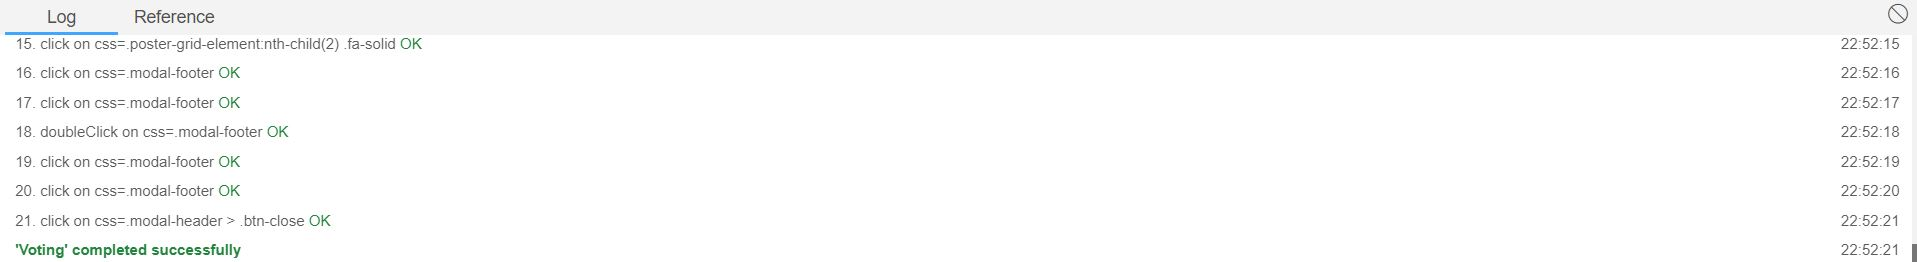
\includegraphics[width=\linewidth]{Slike/votingTest}
			\caption{Prikaz uspješnosti ispitnog slučaja}
		\end{figure}
		
		\begin{lstlisting}
@Test
public void voting() {
	driver.get("https://posterheimer.onrender.com/");
	driver.manage().window().setSize(new Dimension(1536, 824));
	driver.findElement(By.cssSelector(".list-group-item:nth-child(4) > .float-end")).click();
	driver.findElement(By.cssSelector("form")).click();
	driver.findElement(By.id("username")).click();
	driver.findElement(By.id("username")).sendKeys("register2.email@mail.hr");
	driver.findElement(By.id("password")).click();
	driver.findElement(By.id("password")).sendKeys("Lozinka1");
	driver.findElement(By.cssSelector(".btn-primary")).click();
	driver.findElement(By.linkText("Posteri")).click();
	driver.findElement(By.cssSelector(".poster-grid-element:nth-child(1) .fa-solid")).click();
	driver.findElement(By.cssSelector(".btn-success")).click();
	driver.findElement(By.cssSelector(".mx-2")).click();
	driver.findElement(By.cssSelector(".modal-header > .btn-close")).click();
	driver.findElement(By.cssSelector(".poster-grid-element:nth-child(2) .fa-solid")).click();
	driver.findElement(By.cssSelector(".modal-footer")).click();
	driver.findElement(By.cssSelector(".modal-footer")).click();
	{
		WebElement element = driver.findElement(By.cssSelector(".modal-footer"));
		Actions builder = new Actions(driver);
		builder.doubleClick(element).perform();
	}
	driver.findElement(By.cssSelector(".modal-footer")).click();
	driver.findElement(By.cssSelector(".modal-footer")).click();
	driver.findElement(By.cssSelector(".modal-header > .btn-close")).click();
}
		\end{lstlisting}
			
			\eject 
		
		
		\section{Dijagram razmještaja}
			 
			 \indent Dijagram razmještaja prikazuje odnos sklopovskih dijelova sustava međusobno i s programskim rješenjima koja su potrebna za korisnikovu interakciju s aplikacijom. Kao dio udaljene poslužiteljske infrastrukture postoje dva poslužiteljska računala: mrežni poslužitelj i poslužitelj baze podataka. Na mrežnom poslužitelju je aktivan proces programa aplikacije koji komunicira s bazom podataka koja je aktivna na vlastitom poslužitelju. Predviđeno je da korisnik koristi mrežni preglednik na vlastitom računalu za komunikaciju s aplikacijom na mrežnom poslužitelju.
			 
			 \begin{figure} [hbt!]
			 	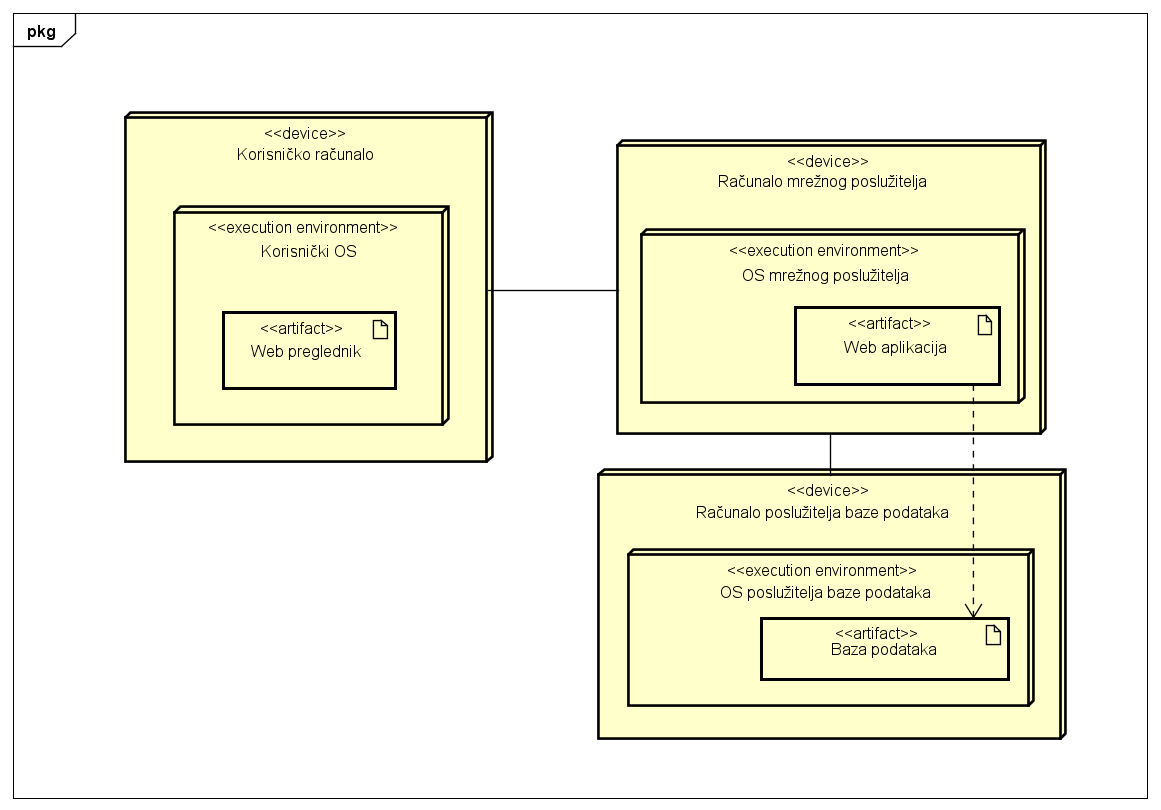
\includegraphics[width=\linewidth]{Slike/DeploymentDiagram}
			 	\caption{Dijagram razmještaja}
			 \end{figure}
			
			\eject 
		
		\section{Upute za puštanje u pogon}
		
			\subsubsection{Kreiranje baze podataka na serveru}
			Pri postavljanju projekta korištena je usluga na računalnom oblaku Render. Nakon izrade korisničkog računa možemo pristupiti opciji "Dashboard", zatim odabiremo opciju "New +" - "PostgreSQL". Unese se ime baze, a ostalo se automatski generira. Odabire se plan plaćanja (besplatna verzija uz više plaćenih), zatim "Create". Time je baza kreirana. Sada ulaskom u dashboard imamo opciju "imebaze-db". Klikom na bazu ulazimo u prozor s informacijama o bazi od kojih su nam neke ključne za spajanje baze s \textit{backend} servisom.
			
			\begin{figure} [H]
				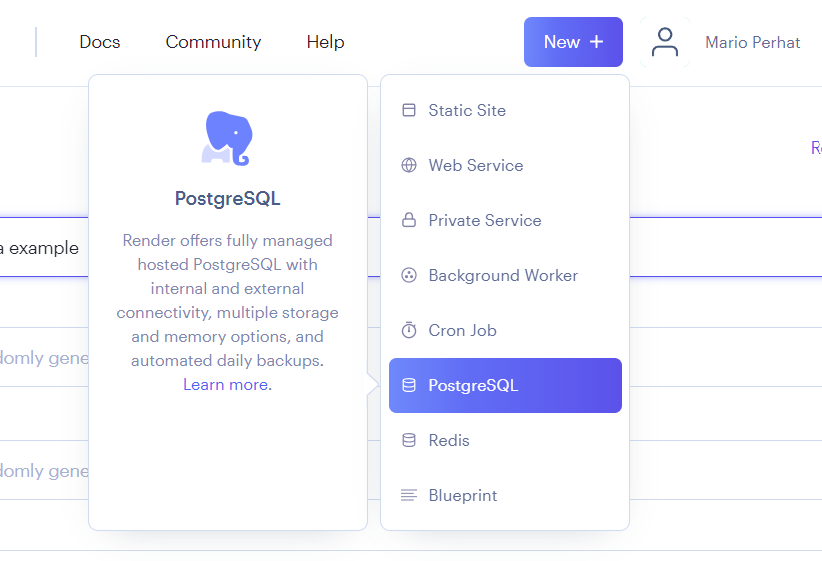
\includegraphics[width=\linewidth]{Slike/Dashboard-New-PostgreSQL}
				\caption{Dashboard-New-PostgreSQL}
			\end{figure}
			
			\begin{figure} [H]
				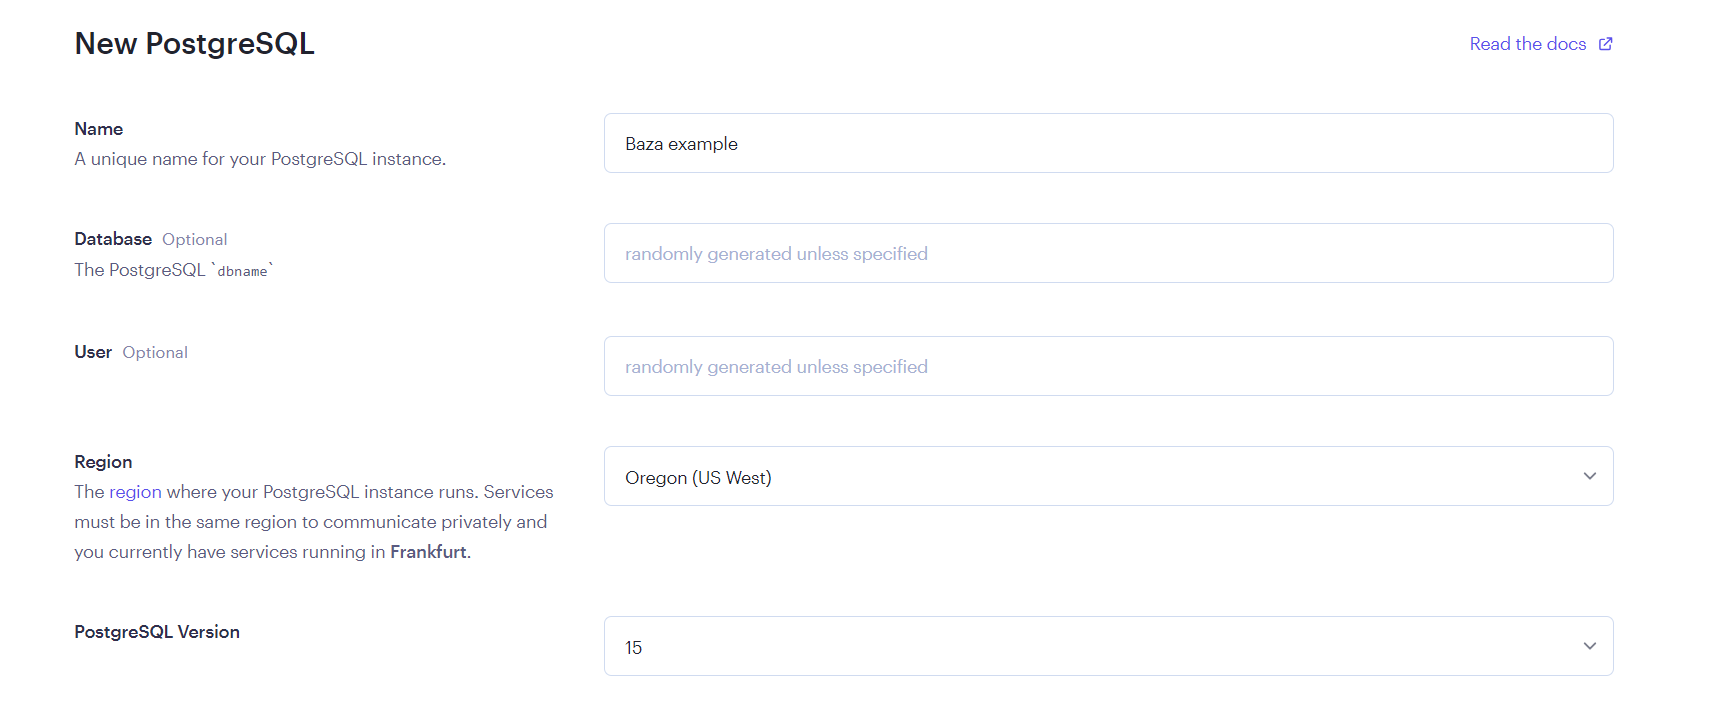
\includegraphics[width=\linewidth]{Slike/Izrada Baze Podataka}
				\caption{Izrada Baze Podataka}
			\end{figure}
			
			\begin{figure} [H]
				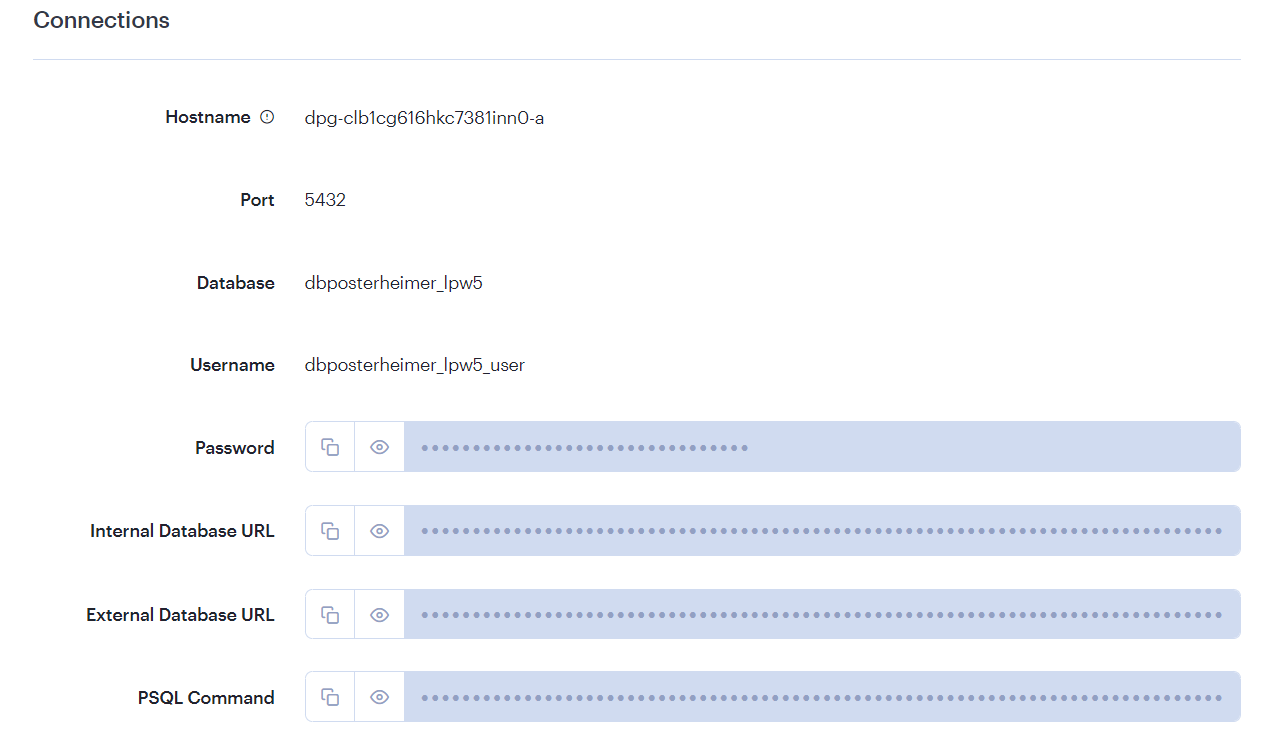
\includegraphics[width=\linewidth]{Slike/Info o Bazi Podataka}
				\caption{Info o Bazi Podataka}
			\end{figure}
			
			\newpage
			\subsubsection{Postavljanje backend servisa na server}
			Prije svega treba pripremiti \textit{backend} za puštanje na server. Dodaje se Dockerfile u direktorij "docker". Sličnim postupkom kao i za bazu, u "Dashboard" kliknemo "New +", zatim "Web Service". Nakon povezivanja git računa dobije se pristup svim repozitorijima kojima račun ima pravo pristupa. Stisnuti "connect" kraj odgovarajućeg projekta.
			\begin{itemize}
			\item Postaviti ime servisa
			\item Root directory postaviti na IzvorniKod/posterheimer-backend
			\item Environment Docker
			\item Region postaviti na Frankfurt
			\item Na dnu proširiti advanced opciju
			\item Dodati potrebne environment varijable
			\item Stisnuti Create Web Service
			\end{itemize}
			Ako je sve dobro postavljeno, nakon što prođe potrebno vrijeme da se sve postavi na server, usluga bi trebala biti "live". 
			
			\begin{figure} [H]
				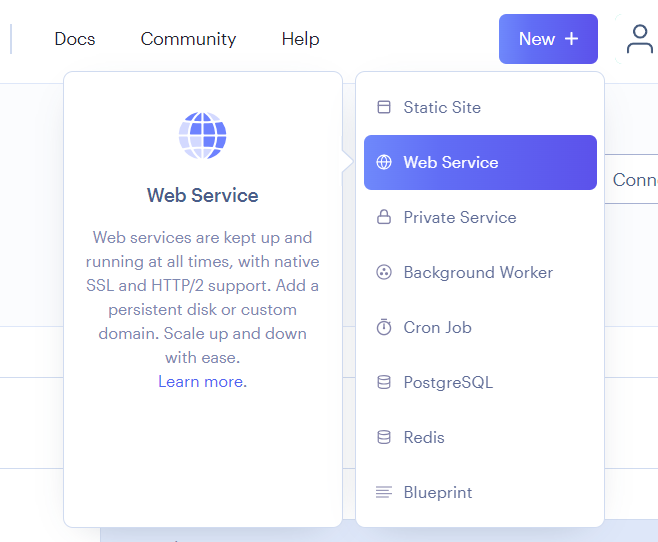
\includegraphics[width=\linewidth]{Slike/Dashboard-New-Web Service}
				\caption{Dashboard-New-Web Service }
			\end{figure}
			
			\begin{figure} [H]
				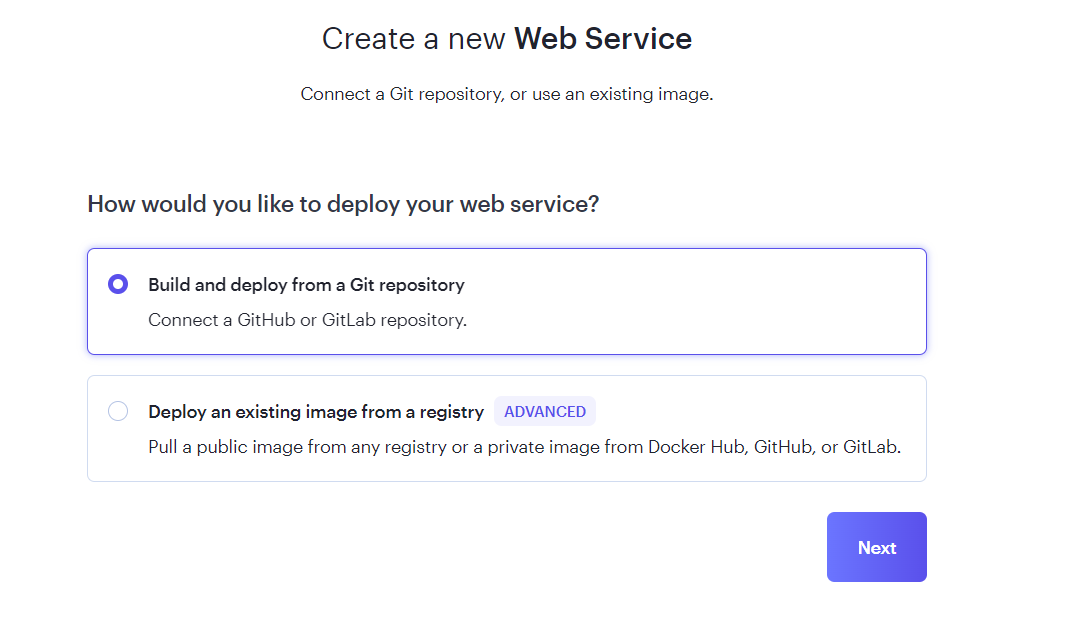
\includegraphics[width=\linewidth]{Slike/Stvaranje iz git repozitorija}
				\caption{Stvaranje iz git repozitorija}
			\end{figure}
			
			\begin{figure} [H]
				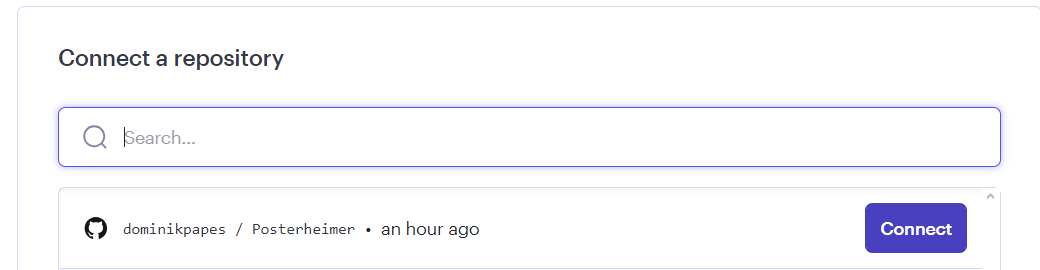
\includegraphics[width=\linewidth]{Slike/Spajanje s repozitorijem}
				\caption{Spajanje s repozitorijem}
			\end{figure}
			
			\begin{figure} [H]
				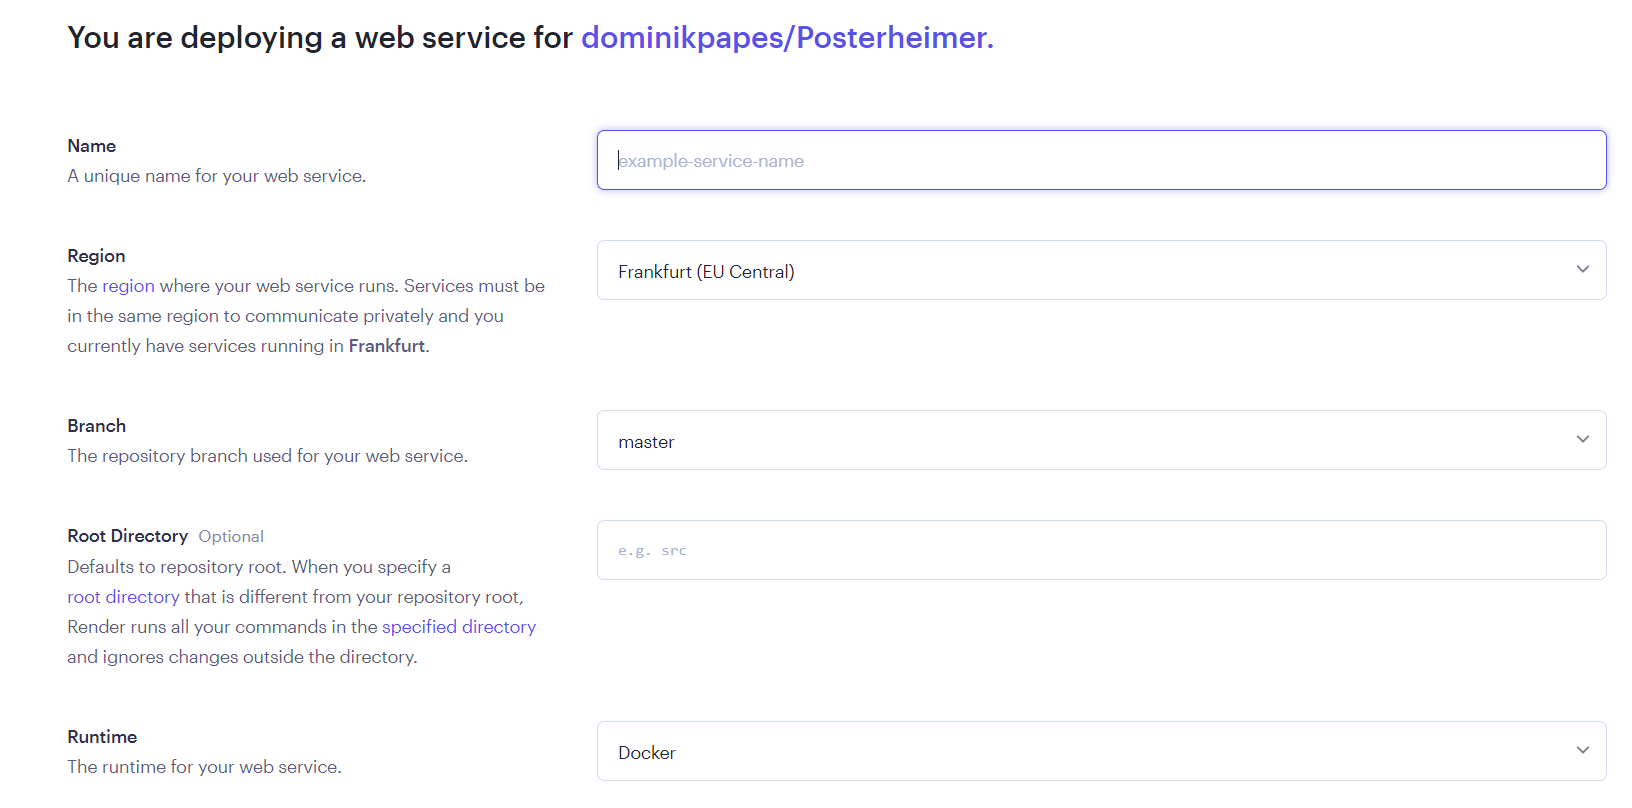
\includegraphics[width=\linewidth]{Slike/Polja za ispunjavanje}
				\caption{Polja za ispunjavanje}
			\end{figure}
			
			\begin{figure} [H]
				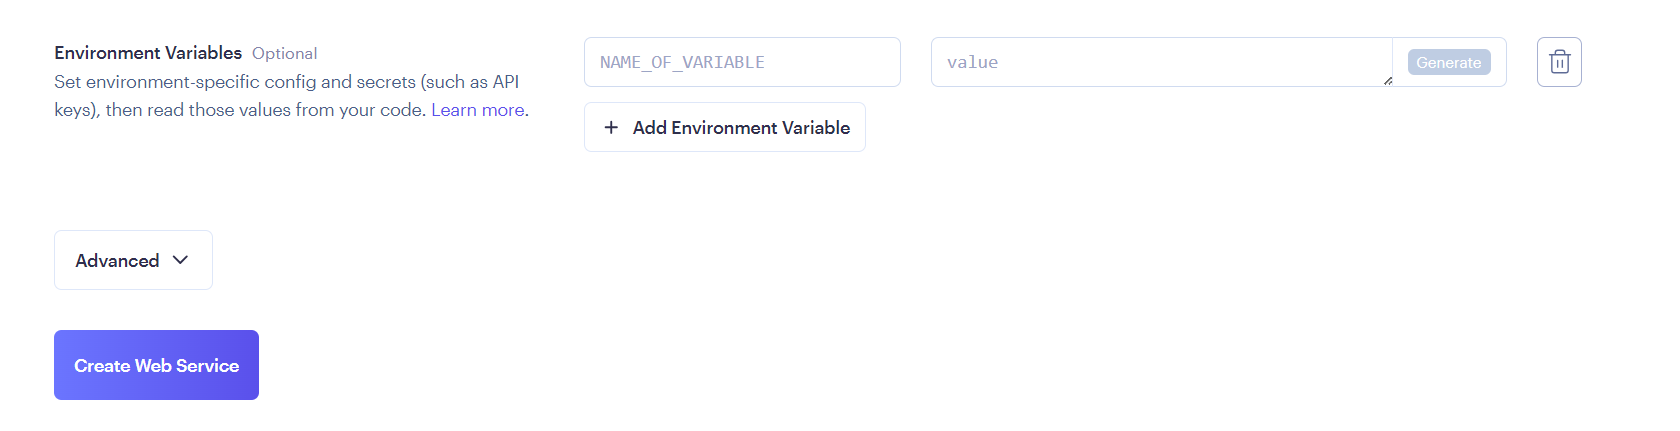
\includegraphics[width=\linewidth]{Slike/Dodavanje Environment varijabli}
				\caption{Dodavanje Environment varijabli}
			\end{figure}
			
			\begin{figure} [H]
				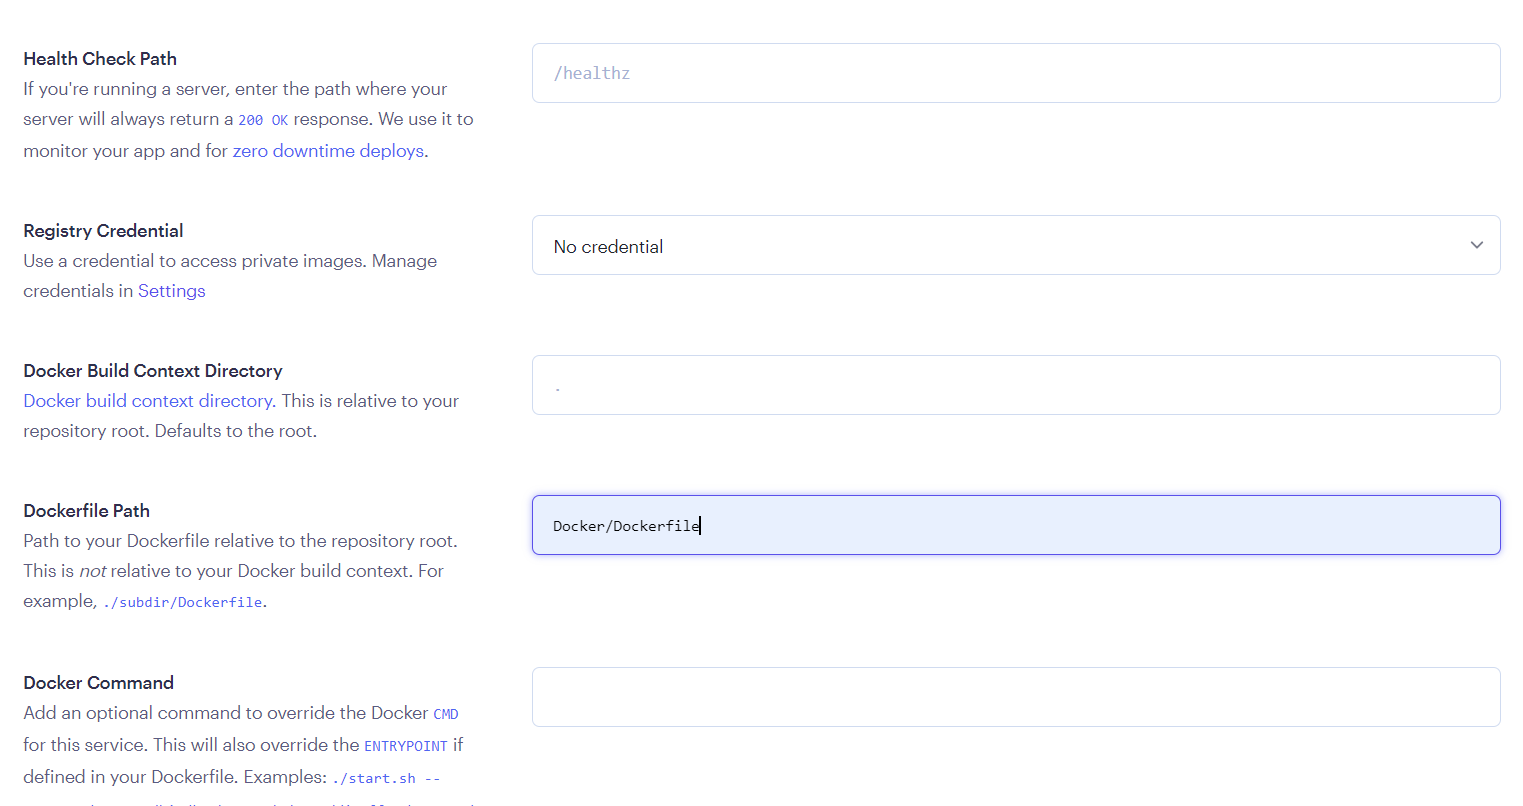
\includegraphics[width=\linewidth]{Slike/Advance-Docker path}
				\caption{Advance-Docker path}
			\end{figure}
			
			\begin{figure} [H]
				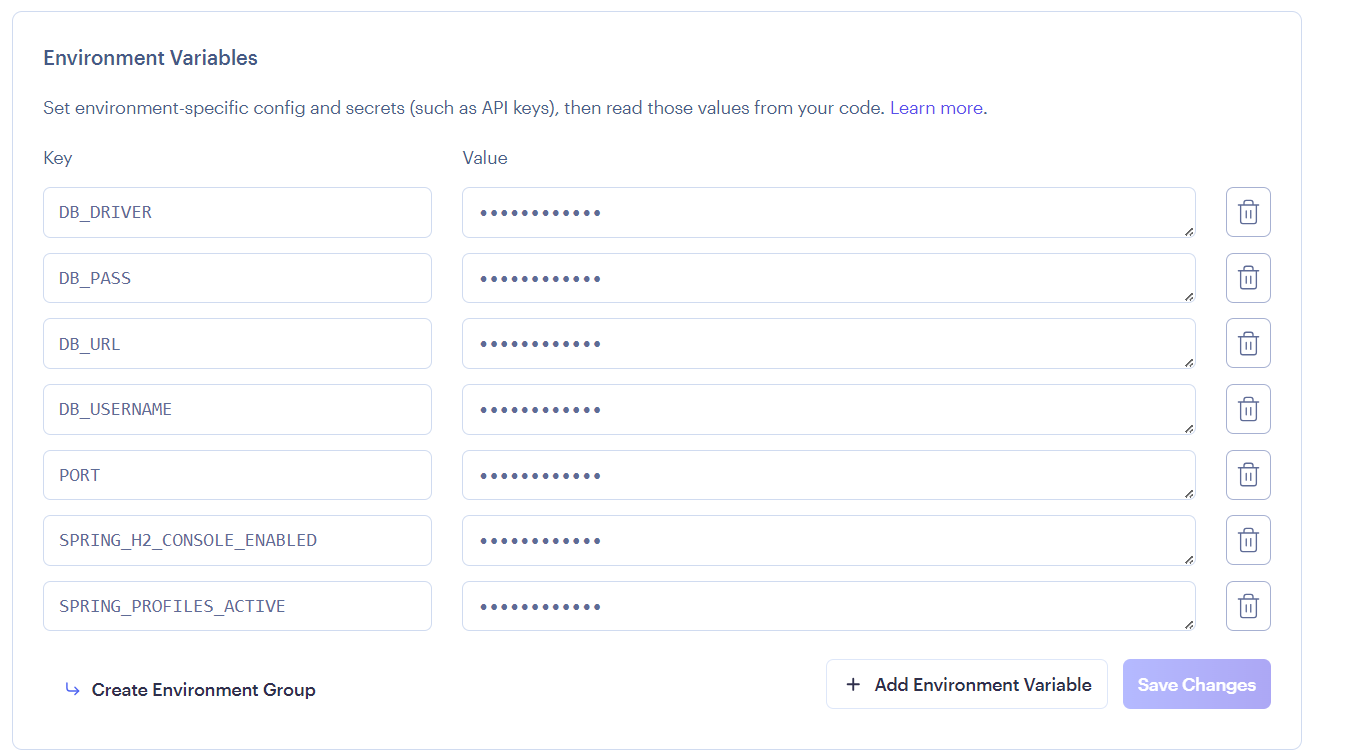
\includegraphics[width=\linewidth]{Slike/Environment varijable}
				\caption{Environment varijable }
			\end{figure}
			
			\newpage
			
			\subsubsection{Puštanje frontenda u pogon}
			Prije svega trebamo imati Github profil s repozitorijem koji sadrži naš kod. U ovom primjeru radi se o repozitoriju Posterheimer. Potom se trebamo prijaviti na Render s pripadajućim Github profilom. U Render Dashboardu odabiremo opciju "New" - "Web Service". 
			
			\begin{figure} [H]
				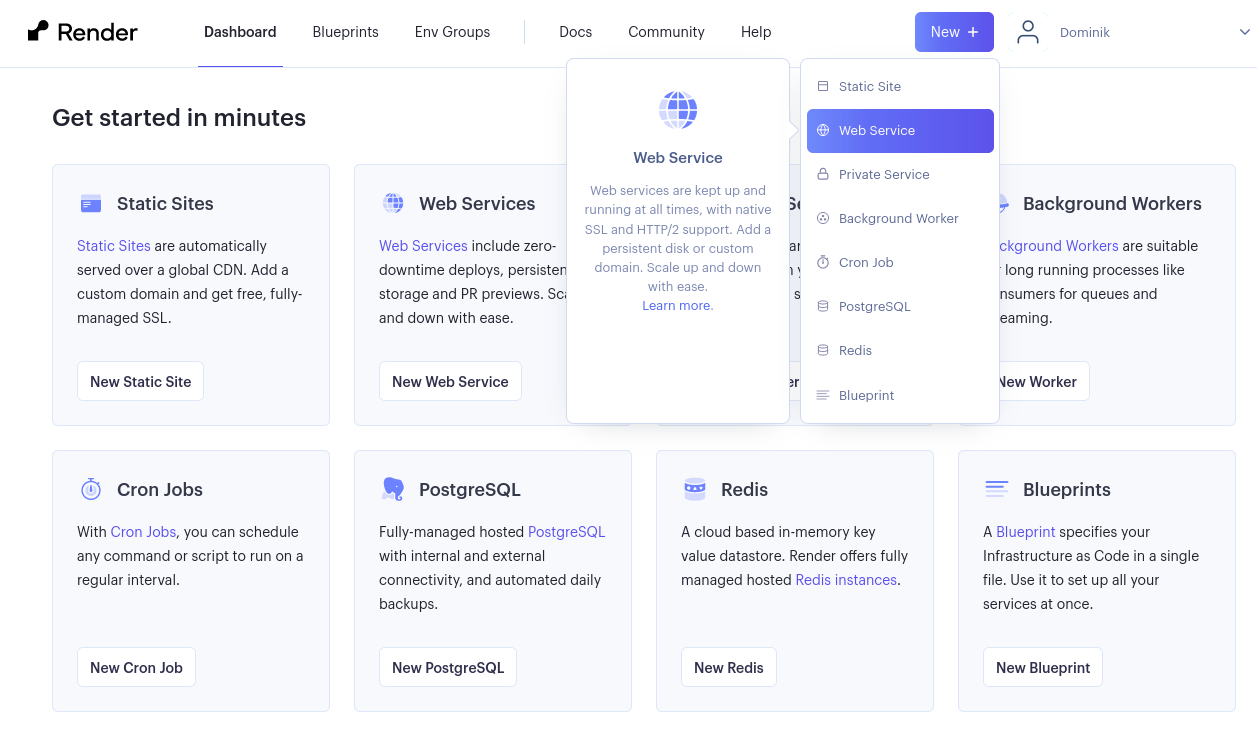
\includegraphics[width=\linewidth]{Slike/Render-Dashboard}
				\caption{Render Dashboard}
			\end{figure}
			
			\newpage
			U sljedećem izborniku odabiremo opciju "Build and deploy from a Git repository"
			
			\begin{figure} [H]
				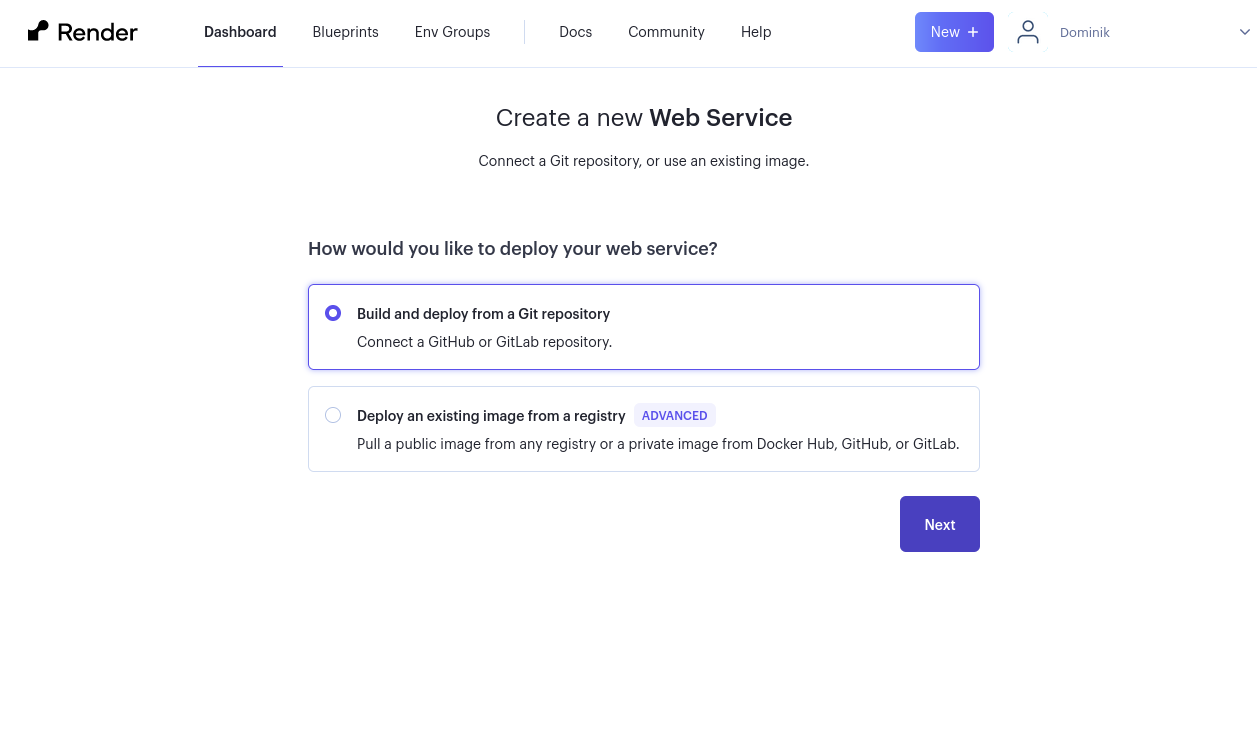
\includegraphics[width=\linewidth]{Slike/Build-and-deploy}
				\caption{Build and deploy}
			\end{figure}
			
			Iz izbornika izabiremo željeni repozitorij i odaberemo opciju "Connect". U sljedećem izborniku odaberemo željeno ime našeg servisa, te regiju u kojoj će se servis pokretati (za europsko tržište odaberemo Frankfurt). Odabiremo granu s koje će se servis pokretati, u našem slučaju to je grana "master". Specifično za pokretanje \textit{frontend} koda želimo da se sve komande pokreću unutar direktorija "IzvorniKod/posterheimer-frontend", stoga ćemo to upisati u polje "Root directory". "Runtime" za naš servis je Node. Komanda izgradnje mora biti "npm install \&\& npm run build". Kod samog pokretanja servisa treba se izvršiti naredba "npm run" start koju upisujemo u Start command polje.
			
			\begin{figure} [H]
				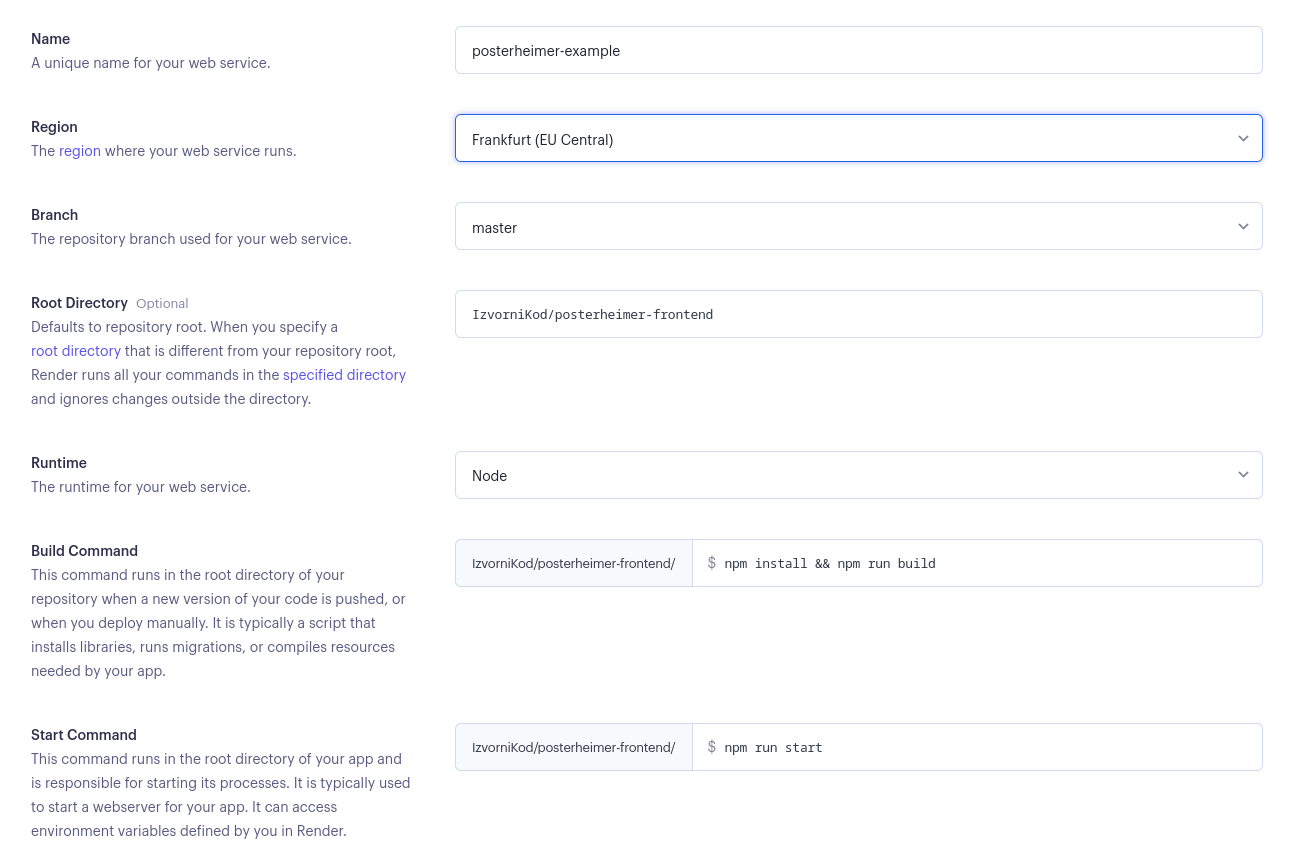
\includegraphics[width=\linewidth]{Slike/Run-Commands}
				\caption{Komande za pokretanje}
			\end{figure}
			
			Možemo odabrati vrstu instance našeg servisa. Postoji besplatna opcija koja nudi najlošije performanse i koju ćemo koristiti za potrebe projekta. Potrebne su nam tri varijable okoline ("Environment variables").
			
			\begin{itemize}
				\item  API\_BASE\_URL = https://posterheimer-service.onrender.com - središnja ruta za sve API pozive prema serveru
				\item HOST = 0.0.0.0 - IP računala na kojem se izvodi servis
				\item  PORT = 3000 - port na kojem računalo sluša
			\end{itemize}
			
			Nakon što smo unijeli sve vrijednosti možemo kliknuti na gumb "Create Web Service" čime će se započeti puštanje aplikacije u pogon. Nakon kratkog čekanja trebali bismo vidjeti poruku "Your service is live!" nakon čega joj možemo pristupiti putem dodijeljenog linka, u ovom slučaju: \textbf{https://posterheimer-example.onrender.com}.
			
			\begin{figure} [H]
				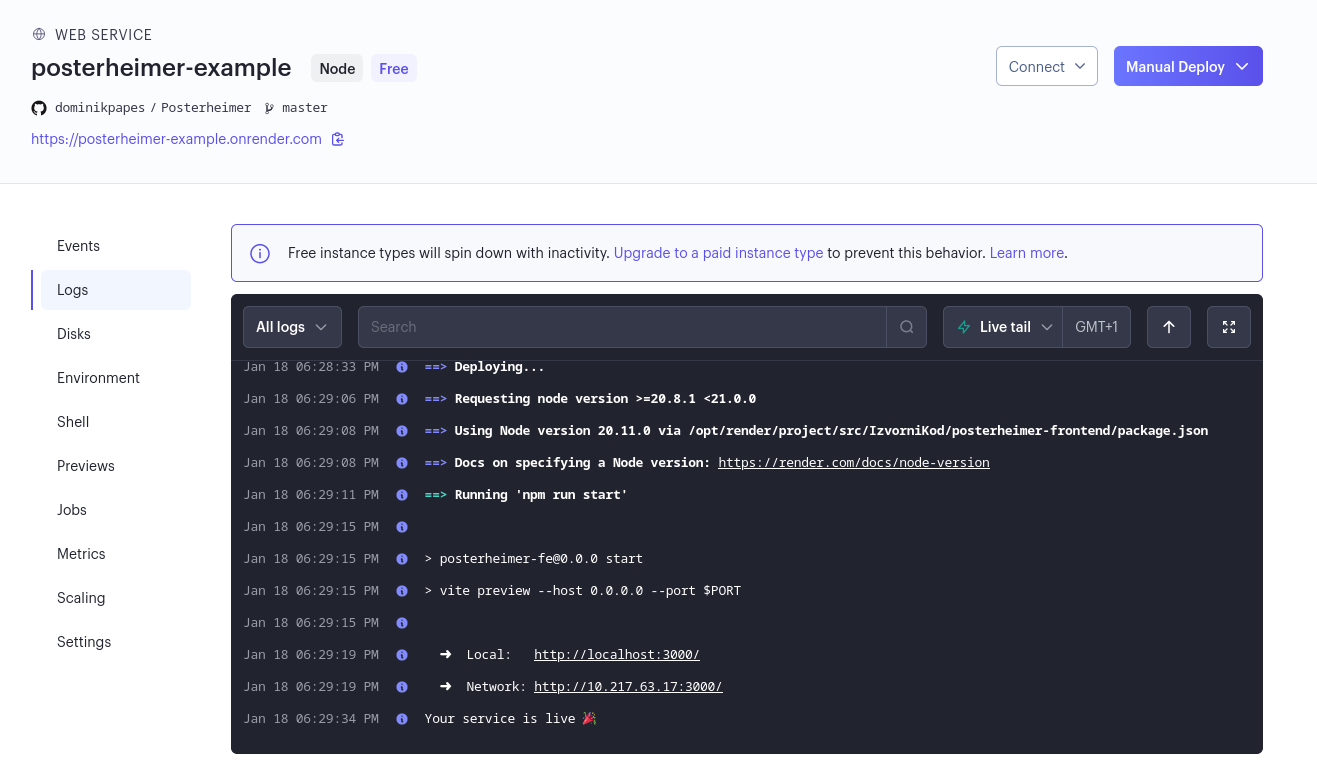
\includegraphics[width=\linewidth]{Slike/Frontend-Deployed}
				\caption{Aplikacija uspješno pokrenuta u pogon}
			\end{figure}
			\eject 